

\chapter{ The Concept of Discretization } \label{sec:Discretization}

The governing ordinary and partial differential equations that occur in many domains of physics describe
\emph{continuous} models. Solving those equations analytically would result in exact continuous solutions. However in practice
a exact analytical solution is not possible and needs to be replaced by a approximation that is found numerically with the aid of computers.
Modern digital computers are only capable of representing a finite and discrete amount of numbers with a finite amount of computational time, memory and storage.
Therefore any continuous model has to be transferred into a discrete model. This process is called \emph{discretization} and for a general spatial or temporal domain $ \Omega $ this is called \emph{domain discretization}. When this transfer happens several different kinds
of error are introduced into the approximate solution. Among others the most important ones are the \textbf{number representation error}, \textbf{roundoff error} and \textbf{truncation error}. For further reading on these error types please refer to pg.8 Press2007.

This section continues the numerical discussion of the CFD equations by focusing on the discretization process. The \emph{continuous} Navier-Stokes equations need to be 
discretized in order to solve them. Since this report focuses on unsteady fluids, the given equations are time-dependend. The differential equation in CFD always have a spatial component and in our case also have time dependent components in them. In the process of discretization these dimensions have to be discretized. This results in approaches for \textbf{spatial} discretization and \textbf{time} discretization. The spatial discretization can be roughly divided into Meshbased and Meshfree methods which are the focus of this report. A very brief outline into time discretization is given to better understand the proceedings of this report.  This Chapter concludes with the spatial discretization methods which are continued in the following Chapters. 


\subsection{Discretization in time}
The discretization of time in differential equations is necessary when time is present in the equations, and furthermore the physical value $ \kappa $ is changing over time.
A subdivision in space, can acquire information from neighbouring divisions in all directions. In contrast to this the discretization in time can only use previously
computed, known values from the past ($ \kappa_{t-1} , ... $) and the present computed value  $ \kappa_{t} $ to predict future values of it. How this is done is not the scope of this
report. Important to mention are two different types of methods: The \emph{explicit} methods and the \emph{implicit} methods. The explicit methods are easier to program
and involve only a small numerical effort per time step $ \delta t $. Unfortunately they are numerically not very stable and for most problems need very small time steps $ \delta t $. The implicit methods are much harder to program since they involve the solution of equation systems. This leads to a much higher numerical effort for one time step $ \delta t $. The benefit of implicit methods is that they are numerically stable and much larger time steps can be chosen. Which method is chosen for a CFD problem depends on the requirements of the solution and e.g. larger time steps are necessary. For further reading on this topic pg.63 Laurien2009 provides a excellent introduction.


\subsection{Discretization in space}
The spatial discretization of a domain $ \Omega $ involves subdividing the continuous spatial distribution of a value (e.g. the distribution of temperature values on a heated iron plate) into finite entities. How this subdivision is done and how their properties like position are defined, depends first of all on what kind of
mathematical perspective one takes concerning the frame of reference. This can be either a Eulerian perspective or a Lagrangian perspective as described in mathperspective. These finite entities that replace this continuum in space can be furthermore bound by general meshes (Meshbased methods) or move freely in the form of particles (Meshfree methods). The main difference between meshbased and meshfree methods lie in the question if a overall geometrical description, aka a \textbf{mesh}, defines the domain discretization or not.
To explain this further please consider Figure PerspVsDisMeth. The Meshbased methods are coloured in red, the Meshfree methods in blue. In general the Meshbased methods, like the Finite Difference and Finite Volume method use a Eulerian perspective and consequently have a static frame of reference. The Finite Element methods are also Meshbased methods, but are a hybrid of the Eulerian perspective and the Lagrangian perspective. A mesh is present, but this mesh actually moves along with the properties in interest. The Smoothed Particle Hydrodynamics method is a pure Lagrangian method with a dynamic frame of reference - the moving particles. 


%Figure Venn of Meshbased and Meshfree
% \begin{figure}[htp]
% \centering

% \def\firstcircle{(0,0) circle (4.0cm)}
% \def\secondcircle{(0:5cm) circle (3.6cm)}

% \begin{tikzpicture}
    
%     % Now we want to highlight the intersection of the first and the
%     % second circle:

% \begin{scope}
% \fill[red] \firstcircle;
% \fill[cyan] \secondcircle;
% \draw [loosely dashed, ultra thick] \firstcircle node [align = center] {Meshbased methods \ \ \ \ \ \ };
% \draw [densely dotted, ultra thick] \secondcircle node [right] {Meshfree methods};
% \end{scope}

%     \begin{scope}
%       \clip \firstcircle;
%       \fill[red]  \secondcircle;

%     \end{scope}

% \draw [loosely dashed, ultra thick] (-3,6) -- (-1.4,6) node[black, right] {The Eulerian perspective}; 
% \draw [dotted, ultra thick] (-3,5) -- (-1.4,5) node[black, right] {The Lagrange perspective}; 

% \draw  node [black, right] at (-0.6,-1.4) {FDM}; 
% \draw  node [black, right] at (-0.6,-2) {FVM}; 
% \draw  node [black, right] at (2.6,0) {FEM}; 

% \draw  node [black, right] at (6,-1) {SPH}; 

% \end{tikzpicture}


% \caption{Perspective vs. Discretization Methods}
% \label{fig:PerspVsDisMeth}
% \end{figure}

\section{Meshes}
\label{sec:general_meshes}
In CFD literature often the term \emph{grid} is also used to refer to a mesh. In this report we will stick to the commonly used term mesh. 

\subsection{Structured and unstructured meshes}




Eulerian Mesh
The Eulerian Mesh incorporates the concept of the sec eulerian descr in its mesh description. Its reference system is fixed in space. Hence the mesh does not move
with the material which is simulated, on the contrary the material moves \emph{through} the Eulerian mesh. Depending on the discretization method the mesh is spatially divided into a certain finite amount of subdomains which are called for example \emph{nodes}, \emph{cells} or \emph{volumes} (FVM). These subdomains remain fixed in space and there position, shape and volume usually does not chance over the time of the simulation. It is mainly used in strong correlation with the Finite Difference and Finite Volume Methods and its properties will be more discussed in the following Chapters. This mesh type is predominantly used in applications where the deformations of a material are not of great concern and the focus lies for example on the flow behaviour. It is yet important to understand that basically all solvable fluid dynamic problems can be discretized with a Eulerian Mesh, even the ones with strong deformations during simulation. This can be achieved with extremly fine meshes. As it will be shown in Chapter problems of fdm this imposes skyrocketing requirements on computation time and memory. Figure EulerMesh illustrates the concept of the Eulerian mesh.
The black, equidistant grid represents the Eulerian mesh, which stays fixed in space throughout a schematic deformation simulation of a material marked in blue. In reality
this coarse mesh would not have had the sufficient discretization to adequately capture even this simple deformation. At least a much finer discretization a the deforming edges would have been necessary. Comparing this simple example to the following Lagrangian Mesh already shows that Eulerian Meshes are not very useful for deforming solid mechanics. The analogy of deformations in solid mechanics are turbulent flows in CFD. Likewise a finer (local) discretization is needed to represent these fine grained physical effects.

\begin{figure}[htb]
\centering
\begin{tabular}{cc}
	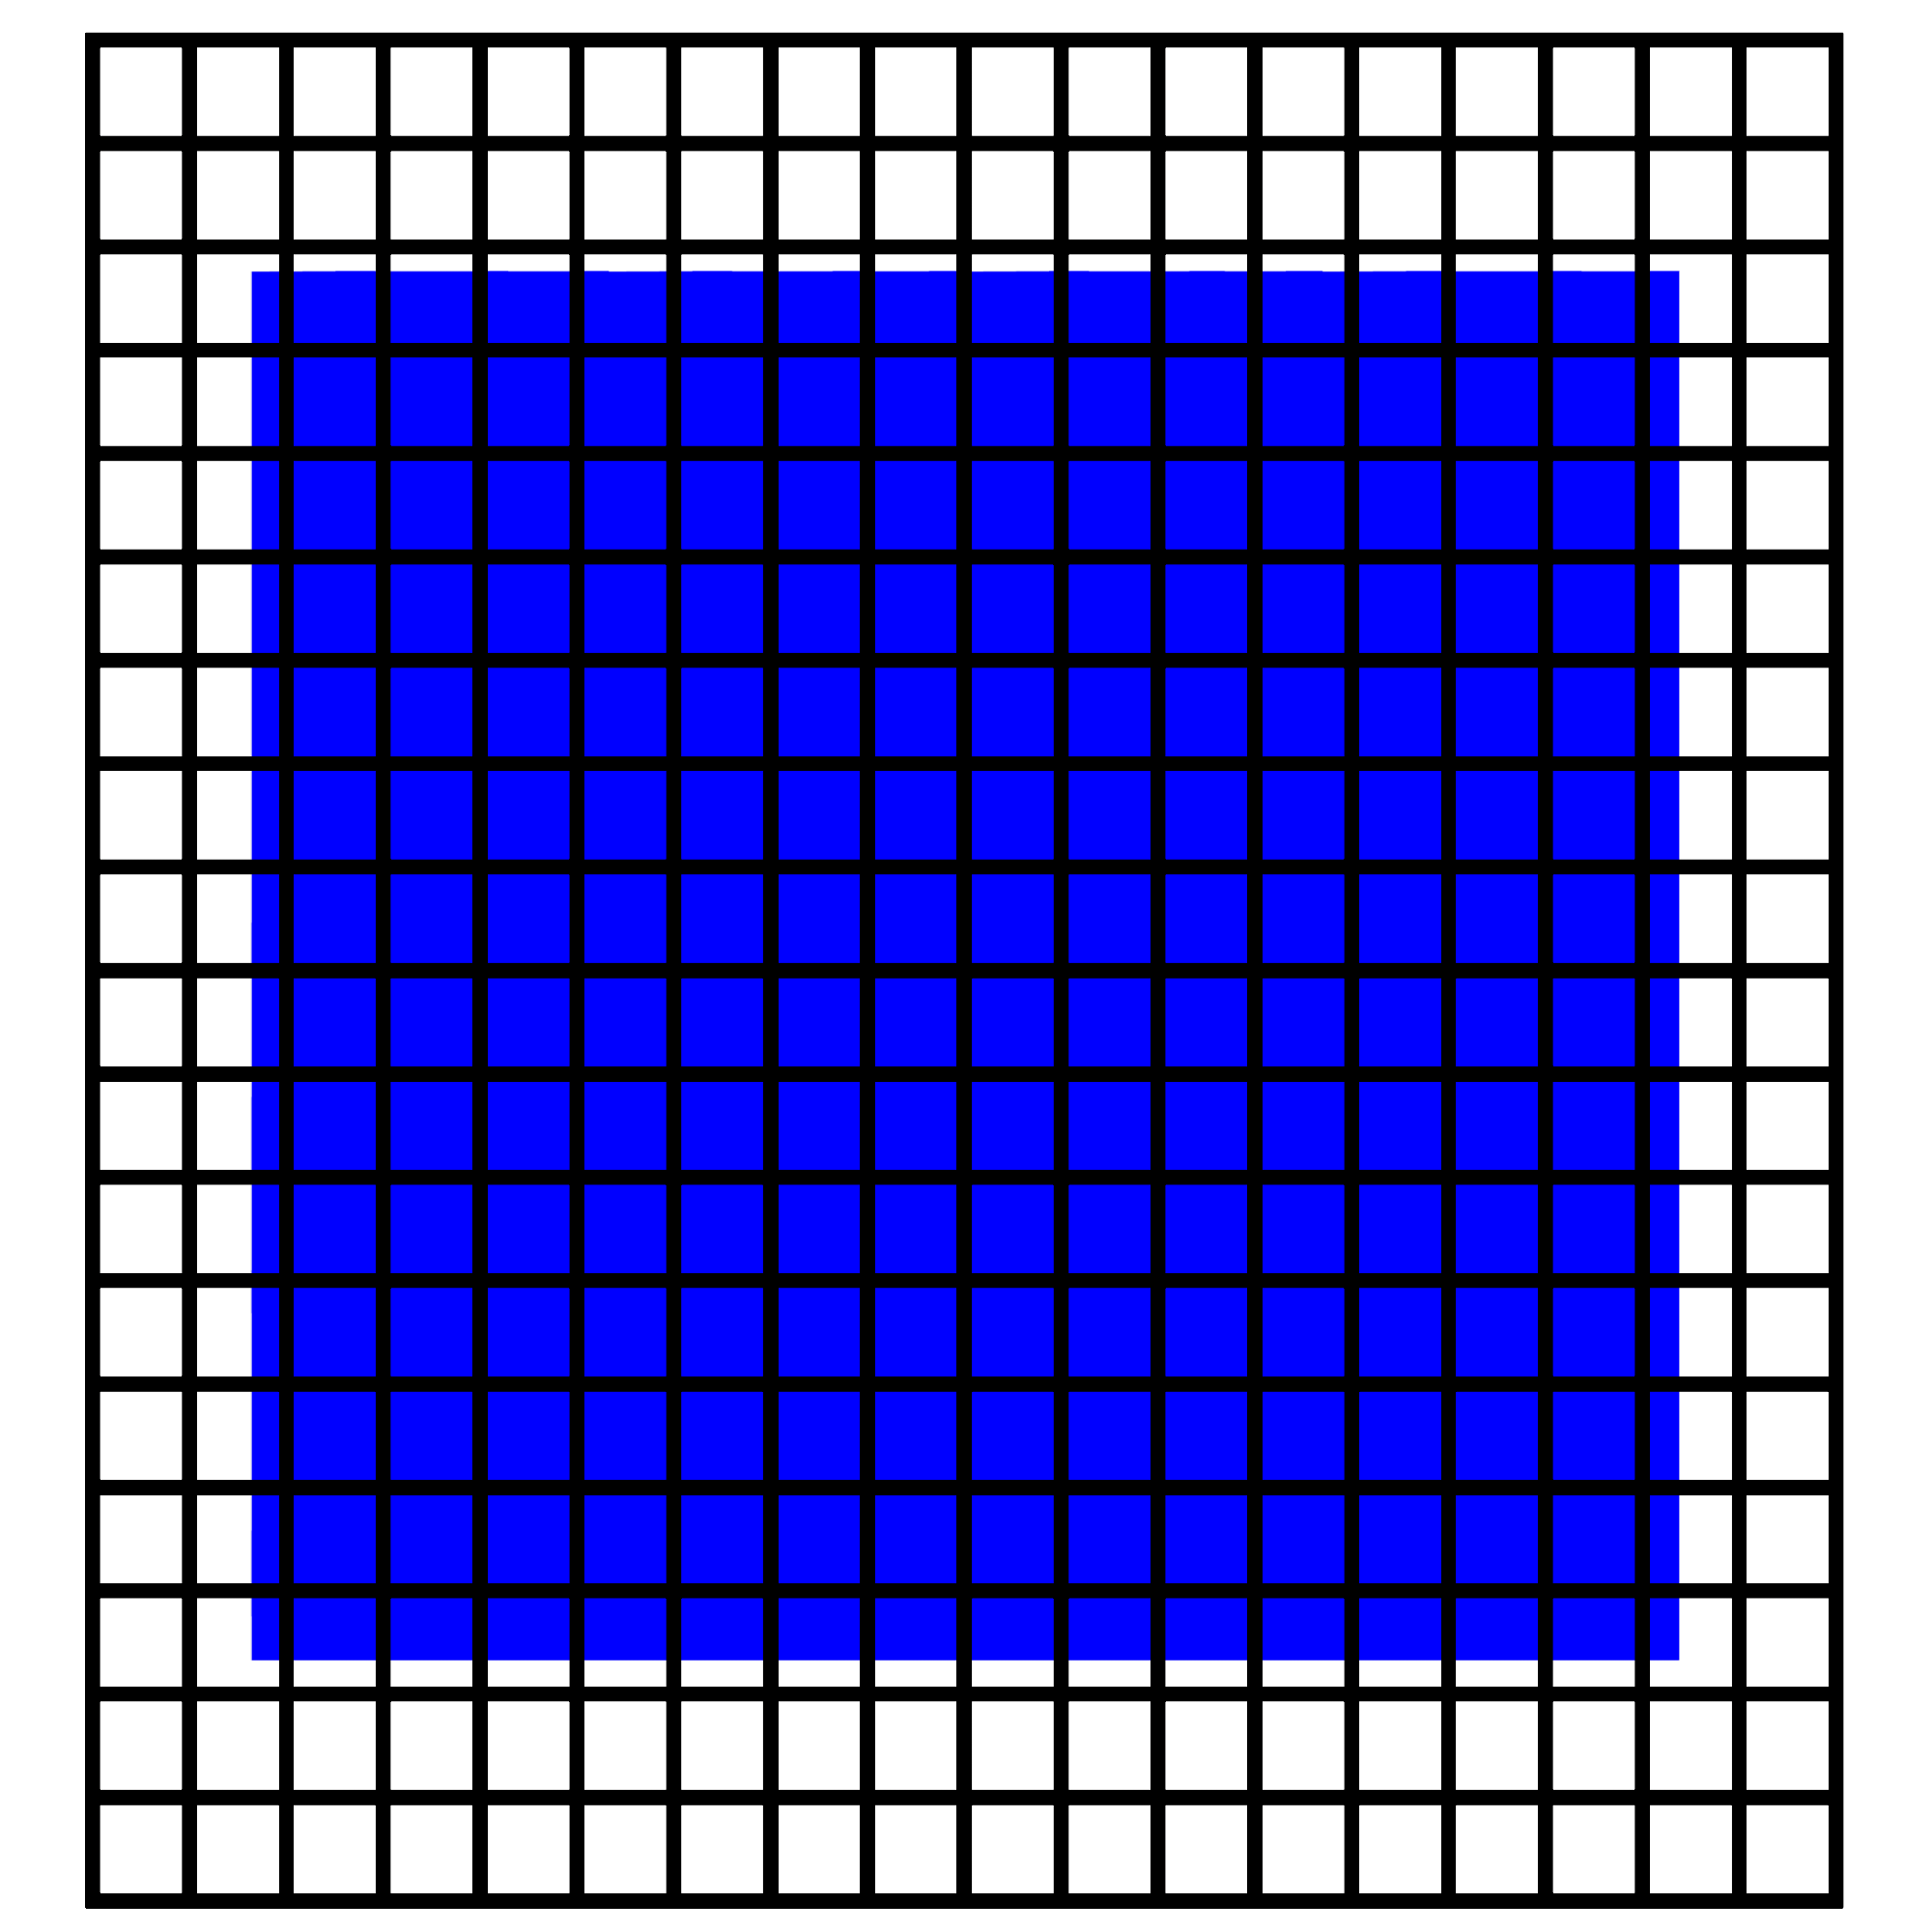
\includegraphics[width=0.4\textwidth]{../figures/eulerian_mesh_movement_001.png}
 &  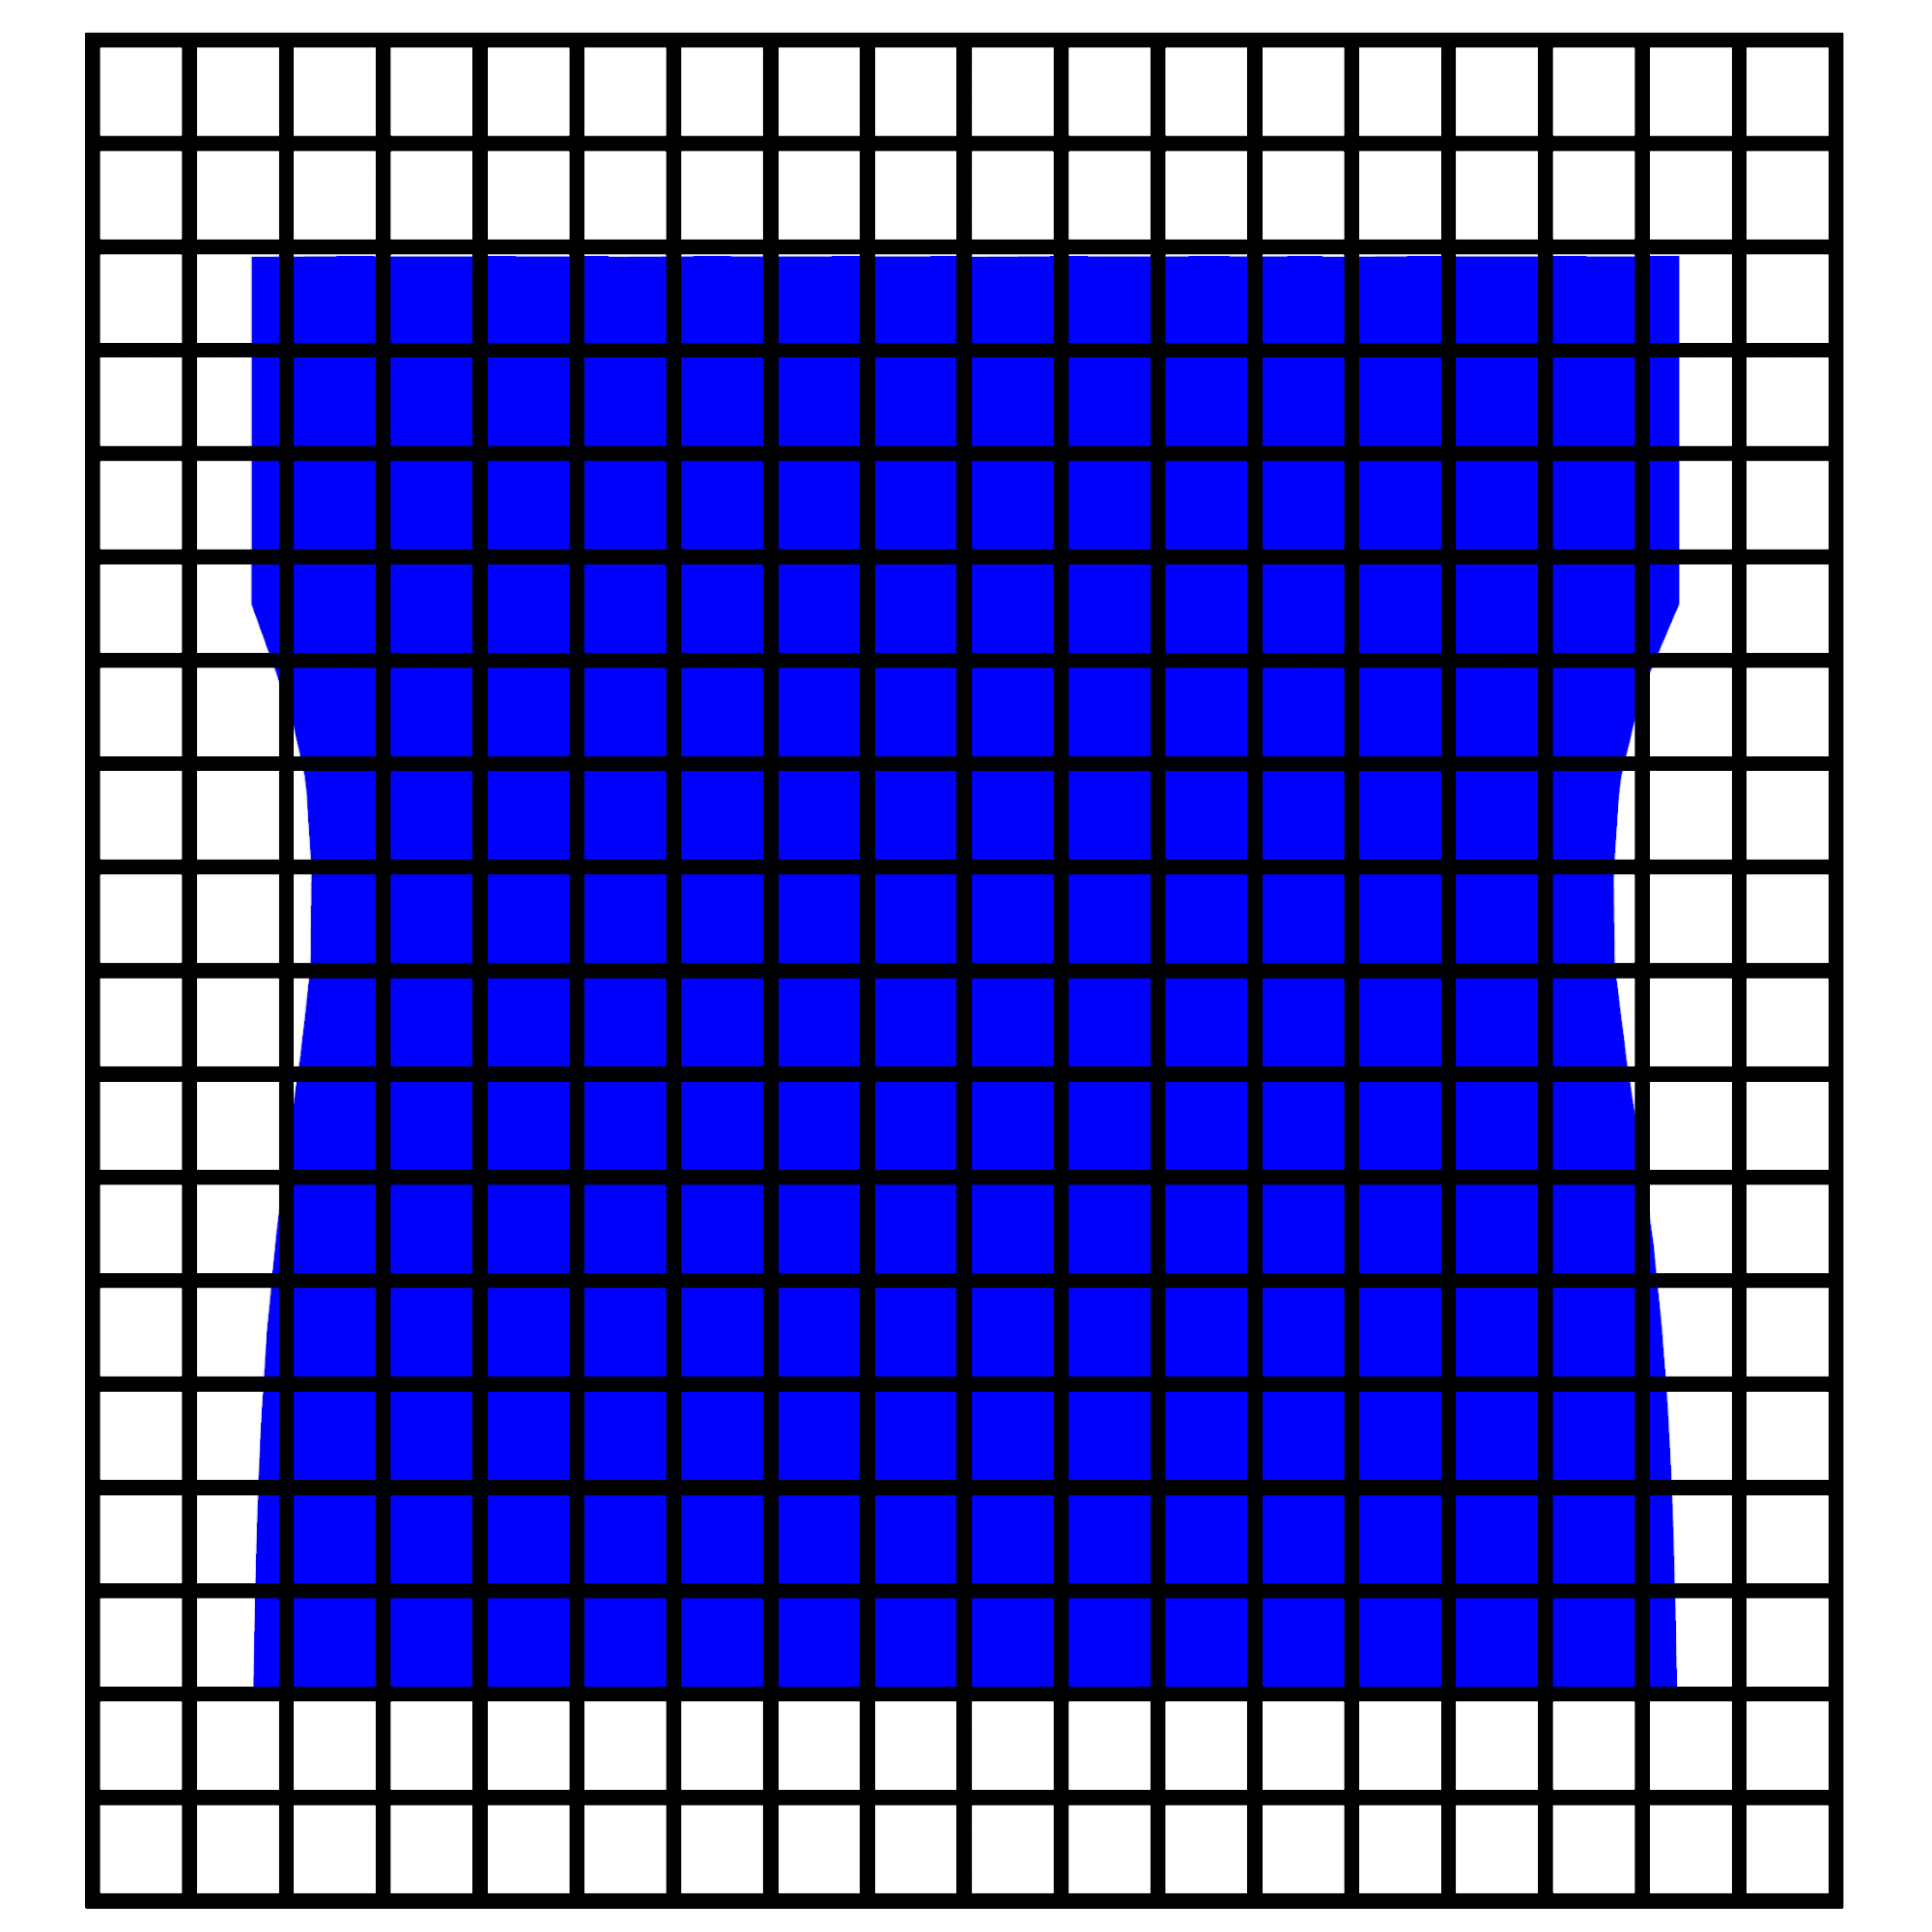
\includegraphics[width=0.4\textwidth]{../figures/eulerian_mesh_movement_002.png} 
 \\

	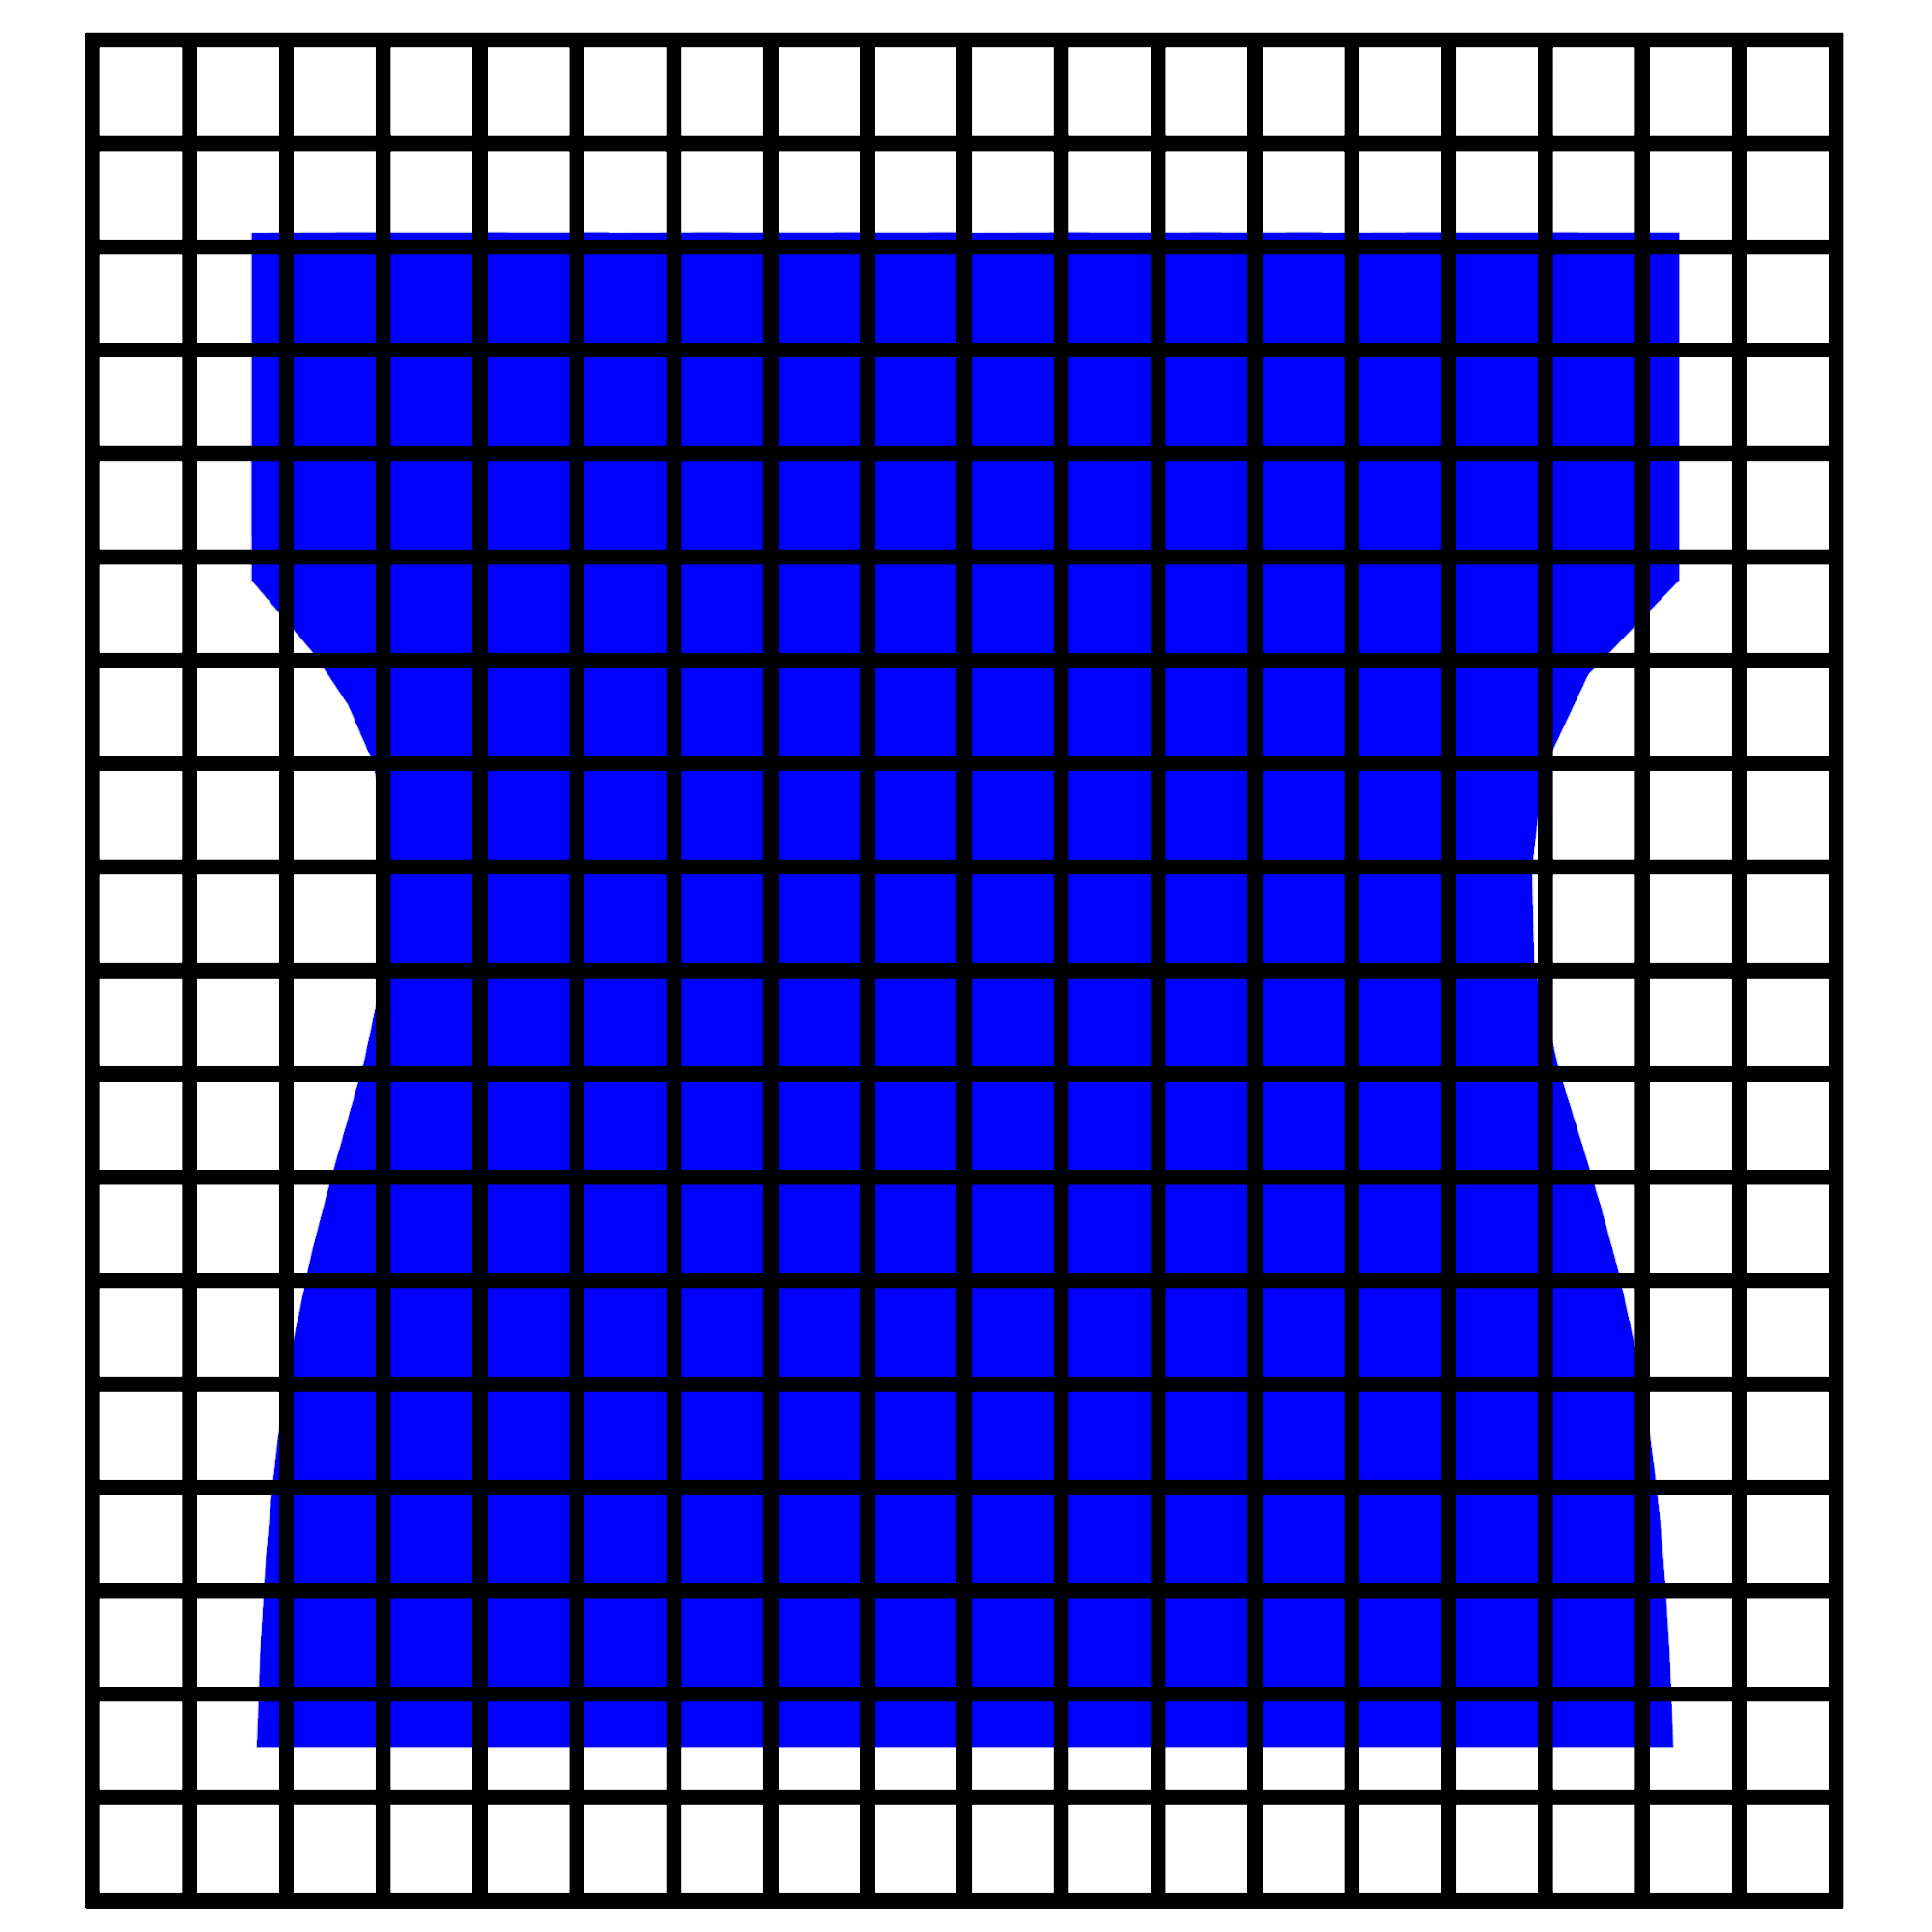
\includegraphics[width=0.4\textwidth]{../figures/eulerian_mesh_movement_003.png} 
 &  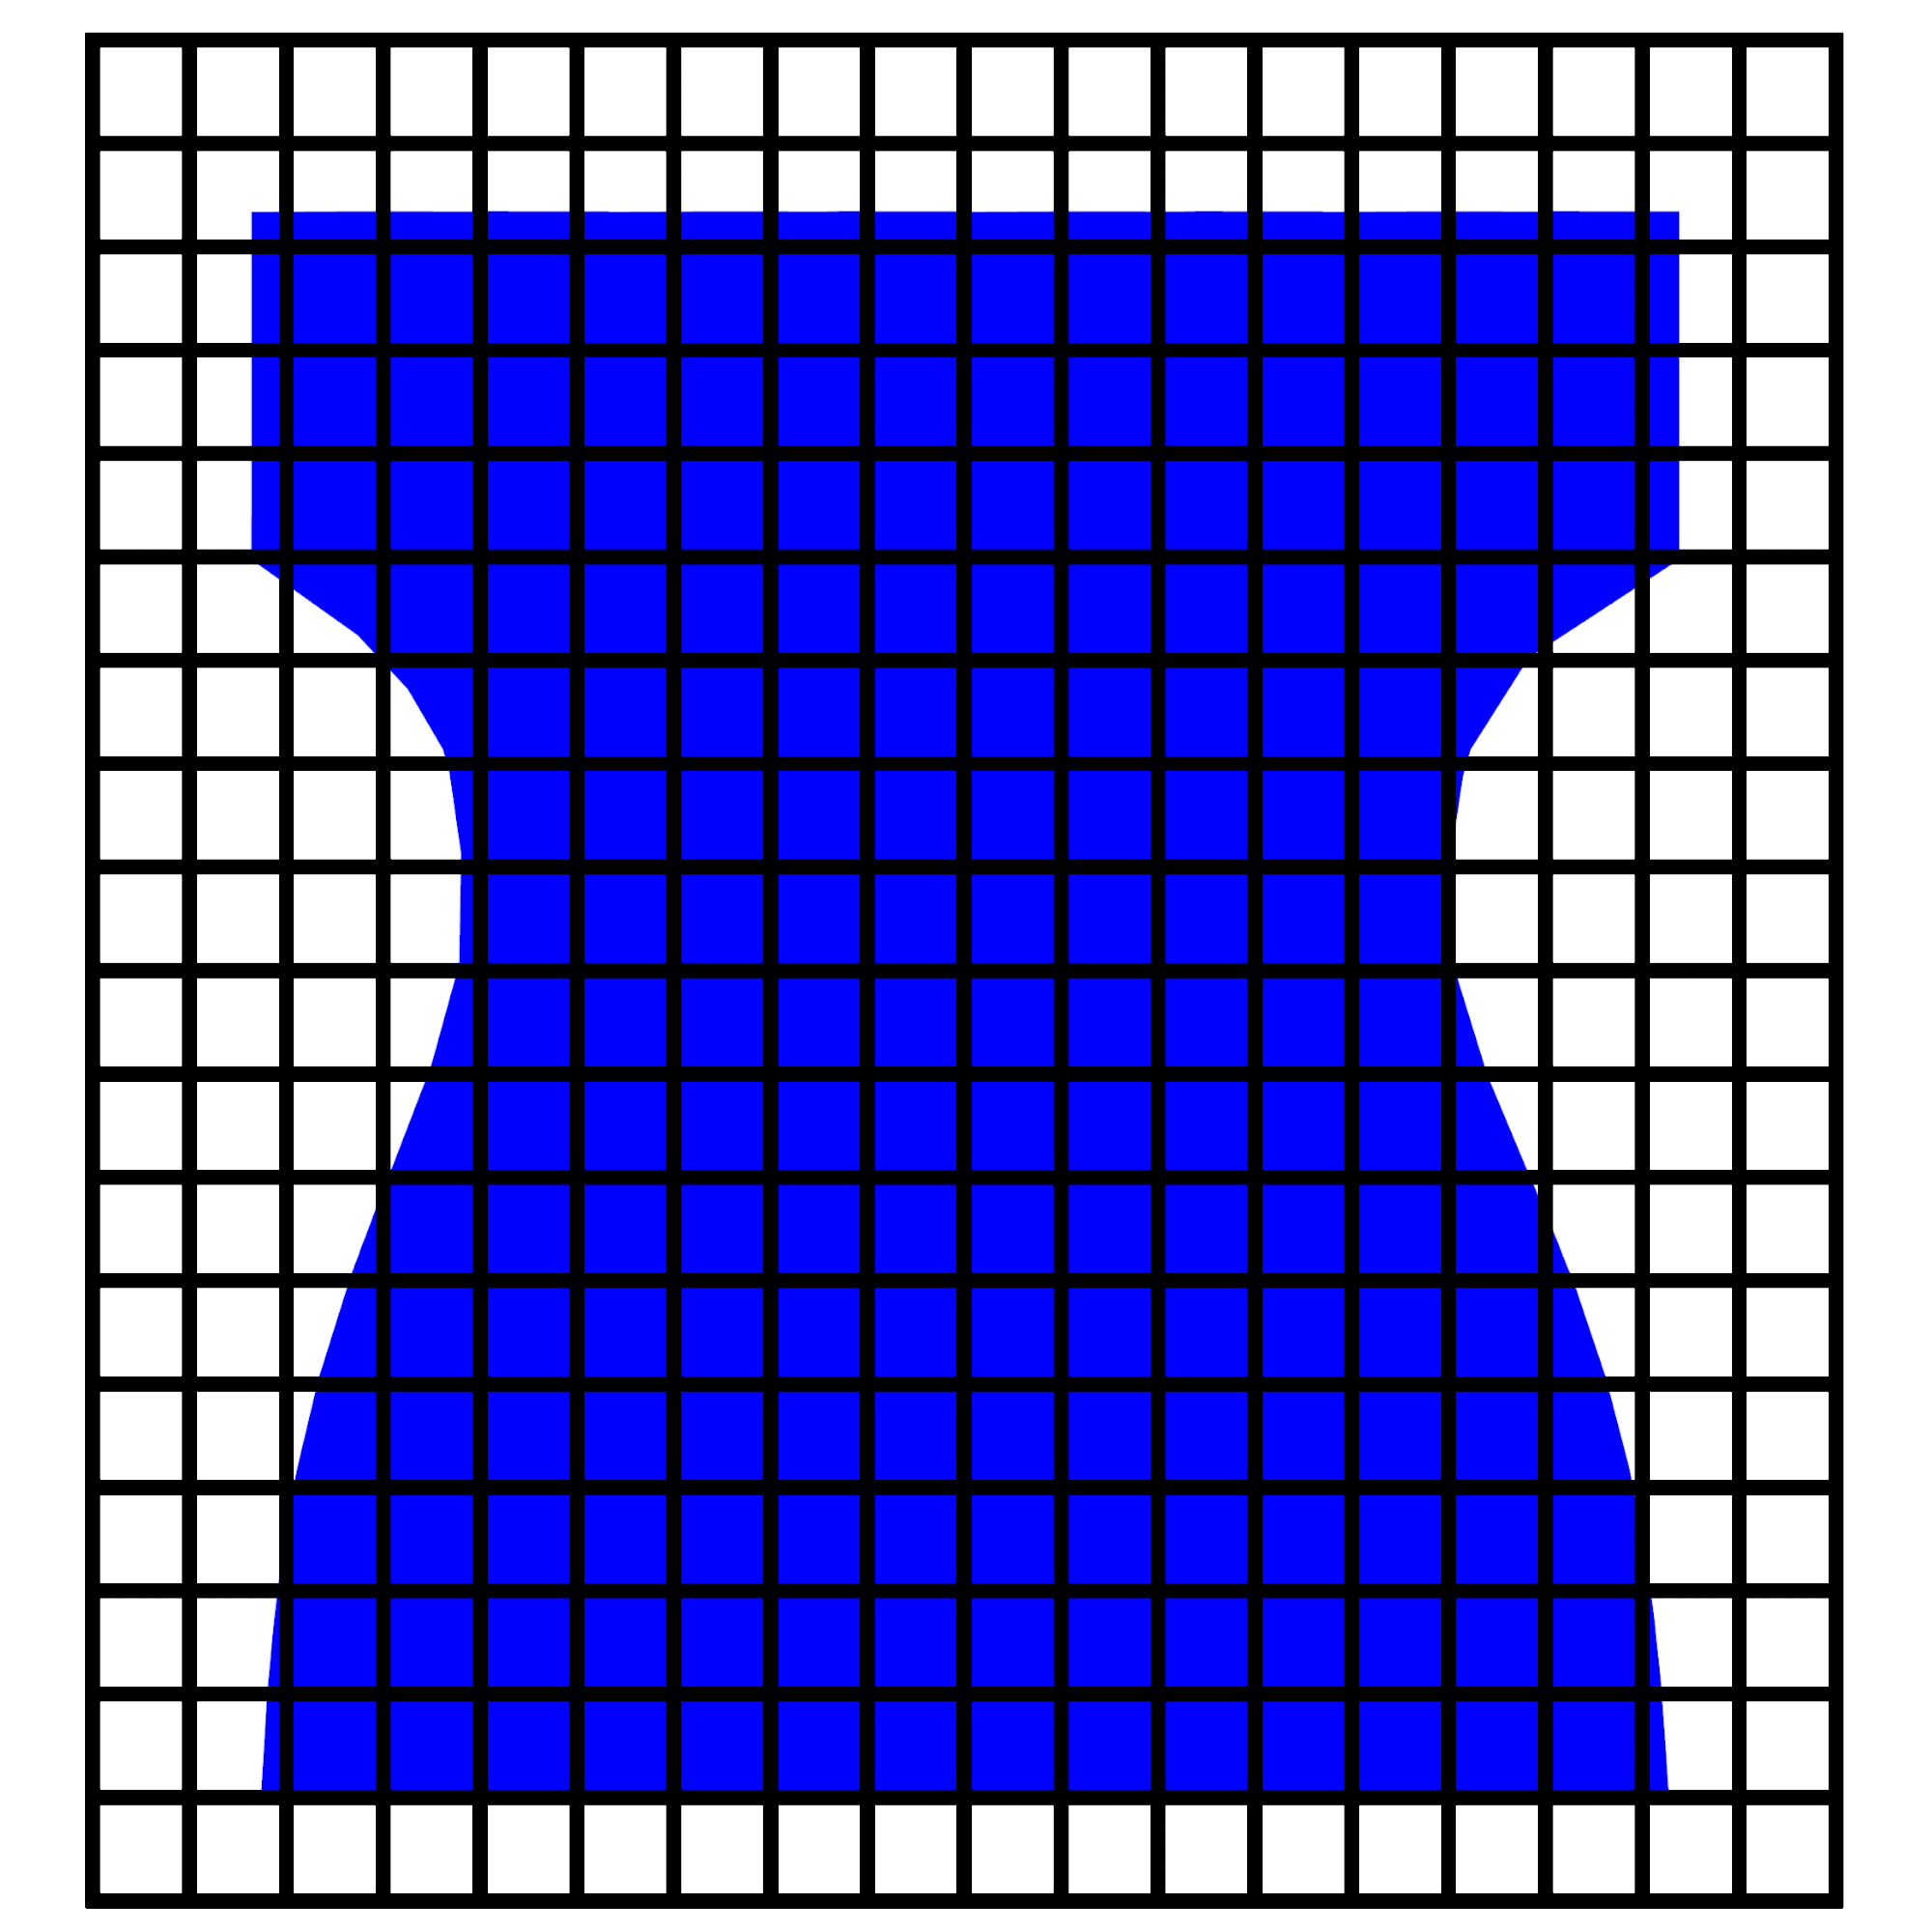
\includegraphics[width=0.4\textwidth]{../figures/eulerian_mesh_movement_004.png}  
 \\

\end{tabular}
\caption[bla]%
{Illustration of static Eulerian Mesh during material deformation \protect\footnotemark}
\label{fig:EulerMesh}
\end{figure}
\footnotetext{Illustration created in Autodesk Maya. This coarse mesh would not be sufficient enough to compute the detail of the deforming blue solid material.}


\subsection{Lagrangian Mesh}

The Lagrangian Mesh type is very similar to the Eulerian Mesh except that it incorporates the idea of the lagrangian descr  into its spatial decomposition: A moving reference system. The mesh itself is clamped to the material and will deform and move accordingly as the material itself. Figure LagMesh
demonstrates such a deformation, in which a stretch behaviour is simulated. The mesh is \emph{body-fitted} to the actual geometry that deforms. In constrast to a Eulerian meshes we can cleary see how the triangular elements of the material deform from the left upper picture to the right lower picture during the simulation. This type of mesh is used in the Finite Element Method for CSM and CFD and has various
advantages over Eulerian Meshes, which will be discussed in Chapteradv of fem. However combining a mesh with the Lagrangian perspective also leads to problems
like remeshing fem. These problems can be overcome by discarding the concept of a mesh description for discretization and creating a meshfree and purer Lagrangian discretization concept with freely moving particles, which is done in Chapter \ref{Chapter 5}. For further reading please refer to Bennett2006.


\begin{figure}[htb]
\centering
\begin{tabular}{cc}
	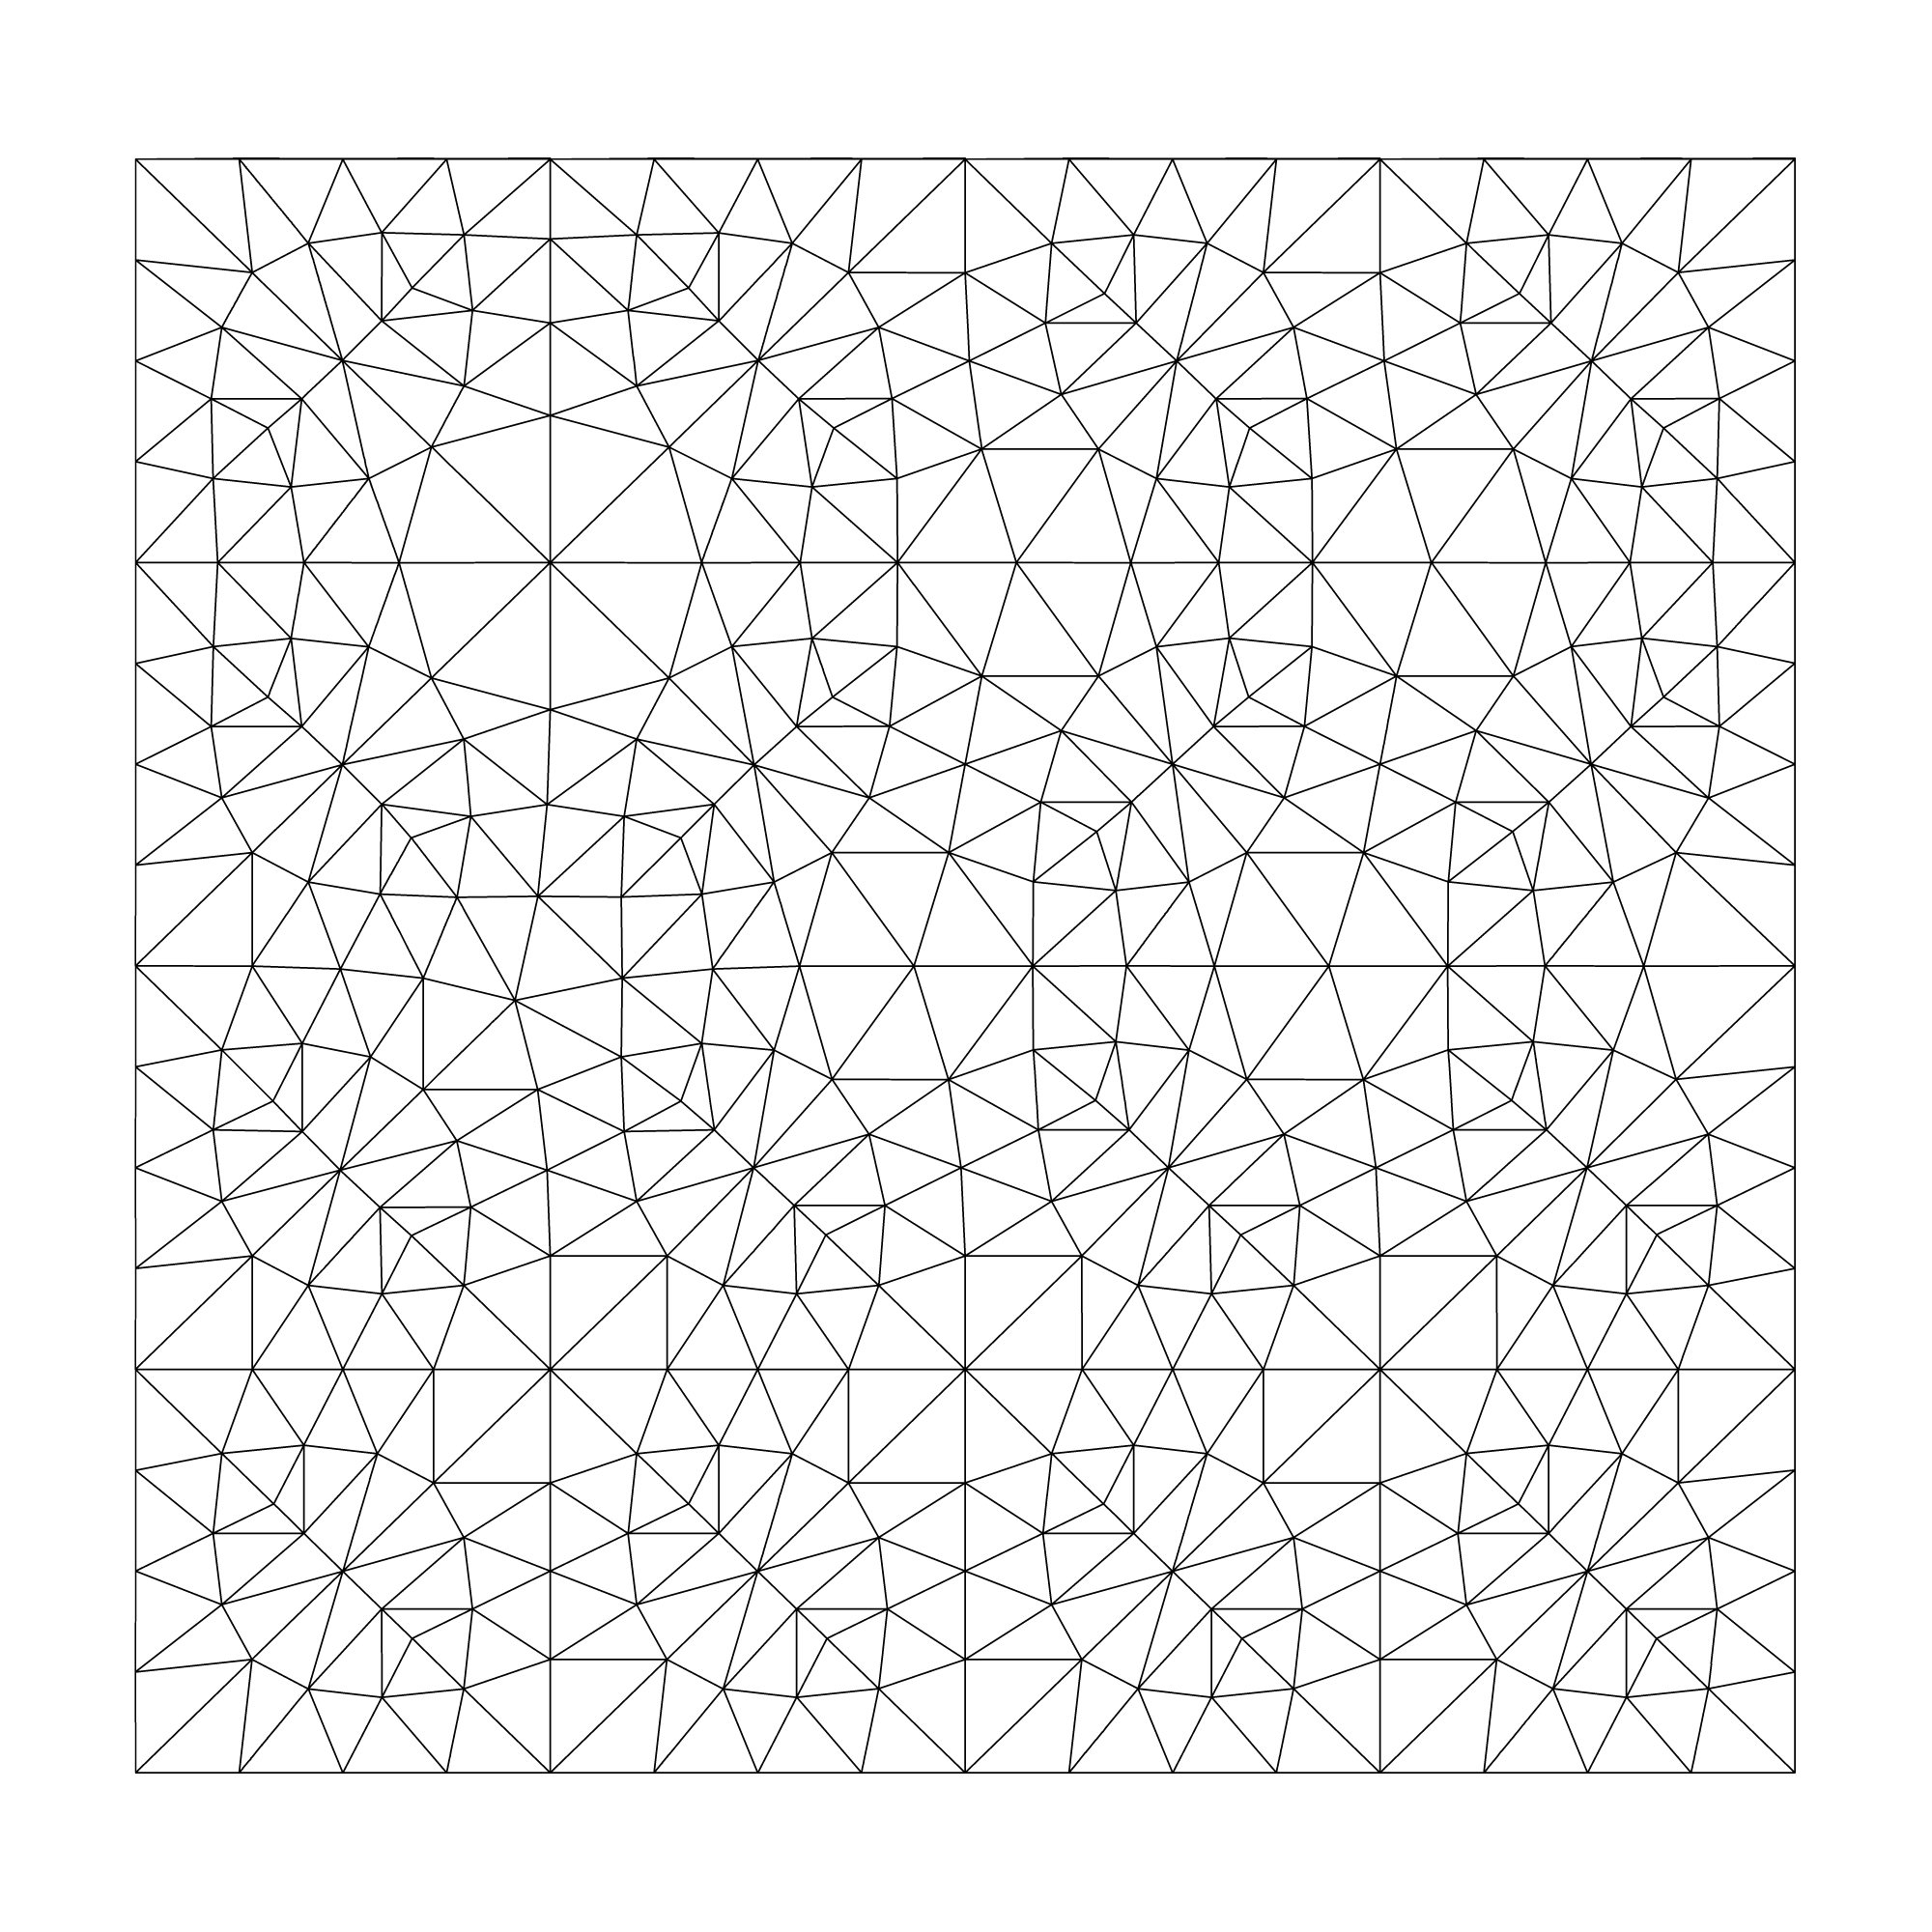
\includegraphics[width=0.4\textwidth]{../figures/lagrangian_mesh_movement_001.png}
 &  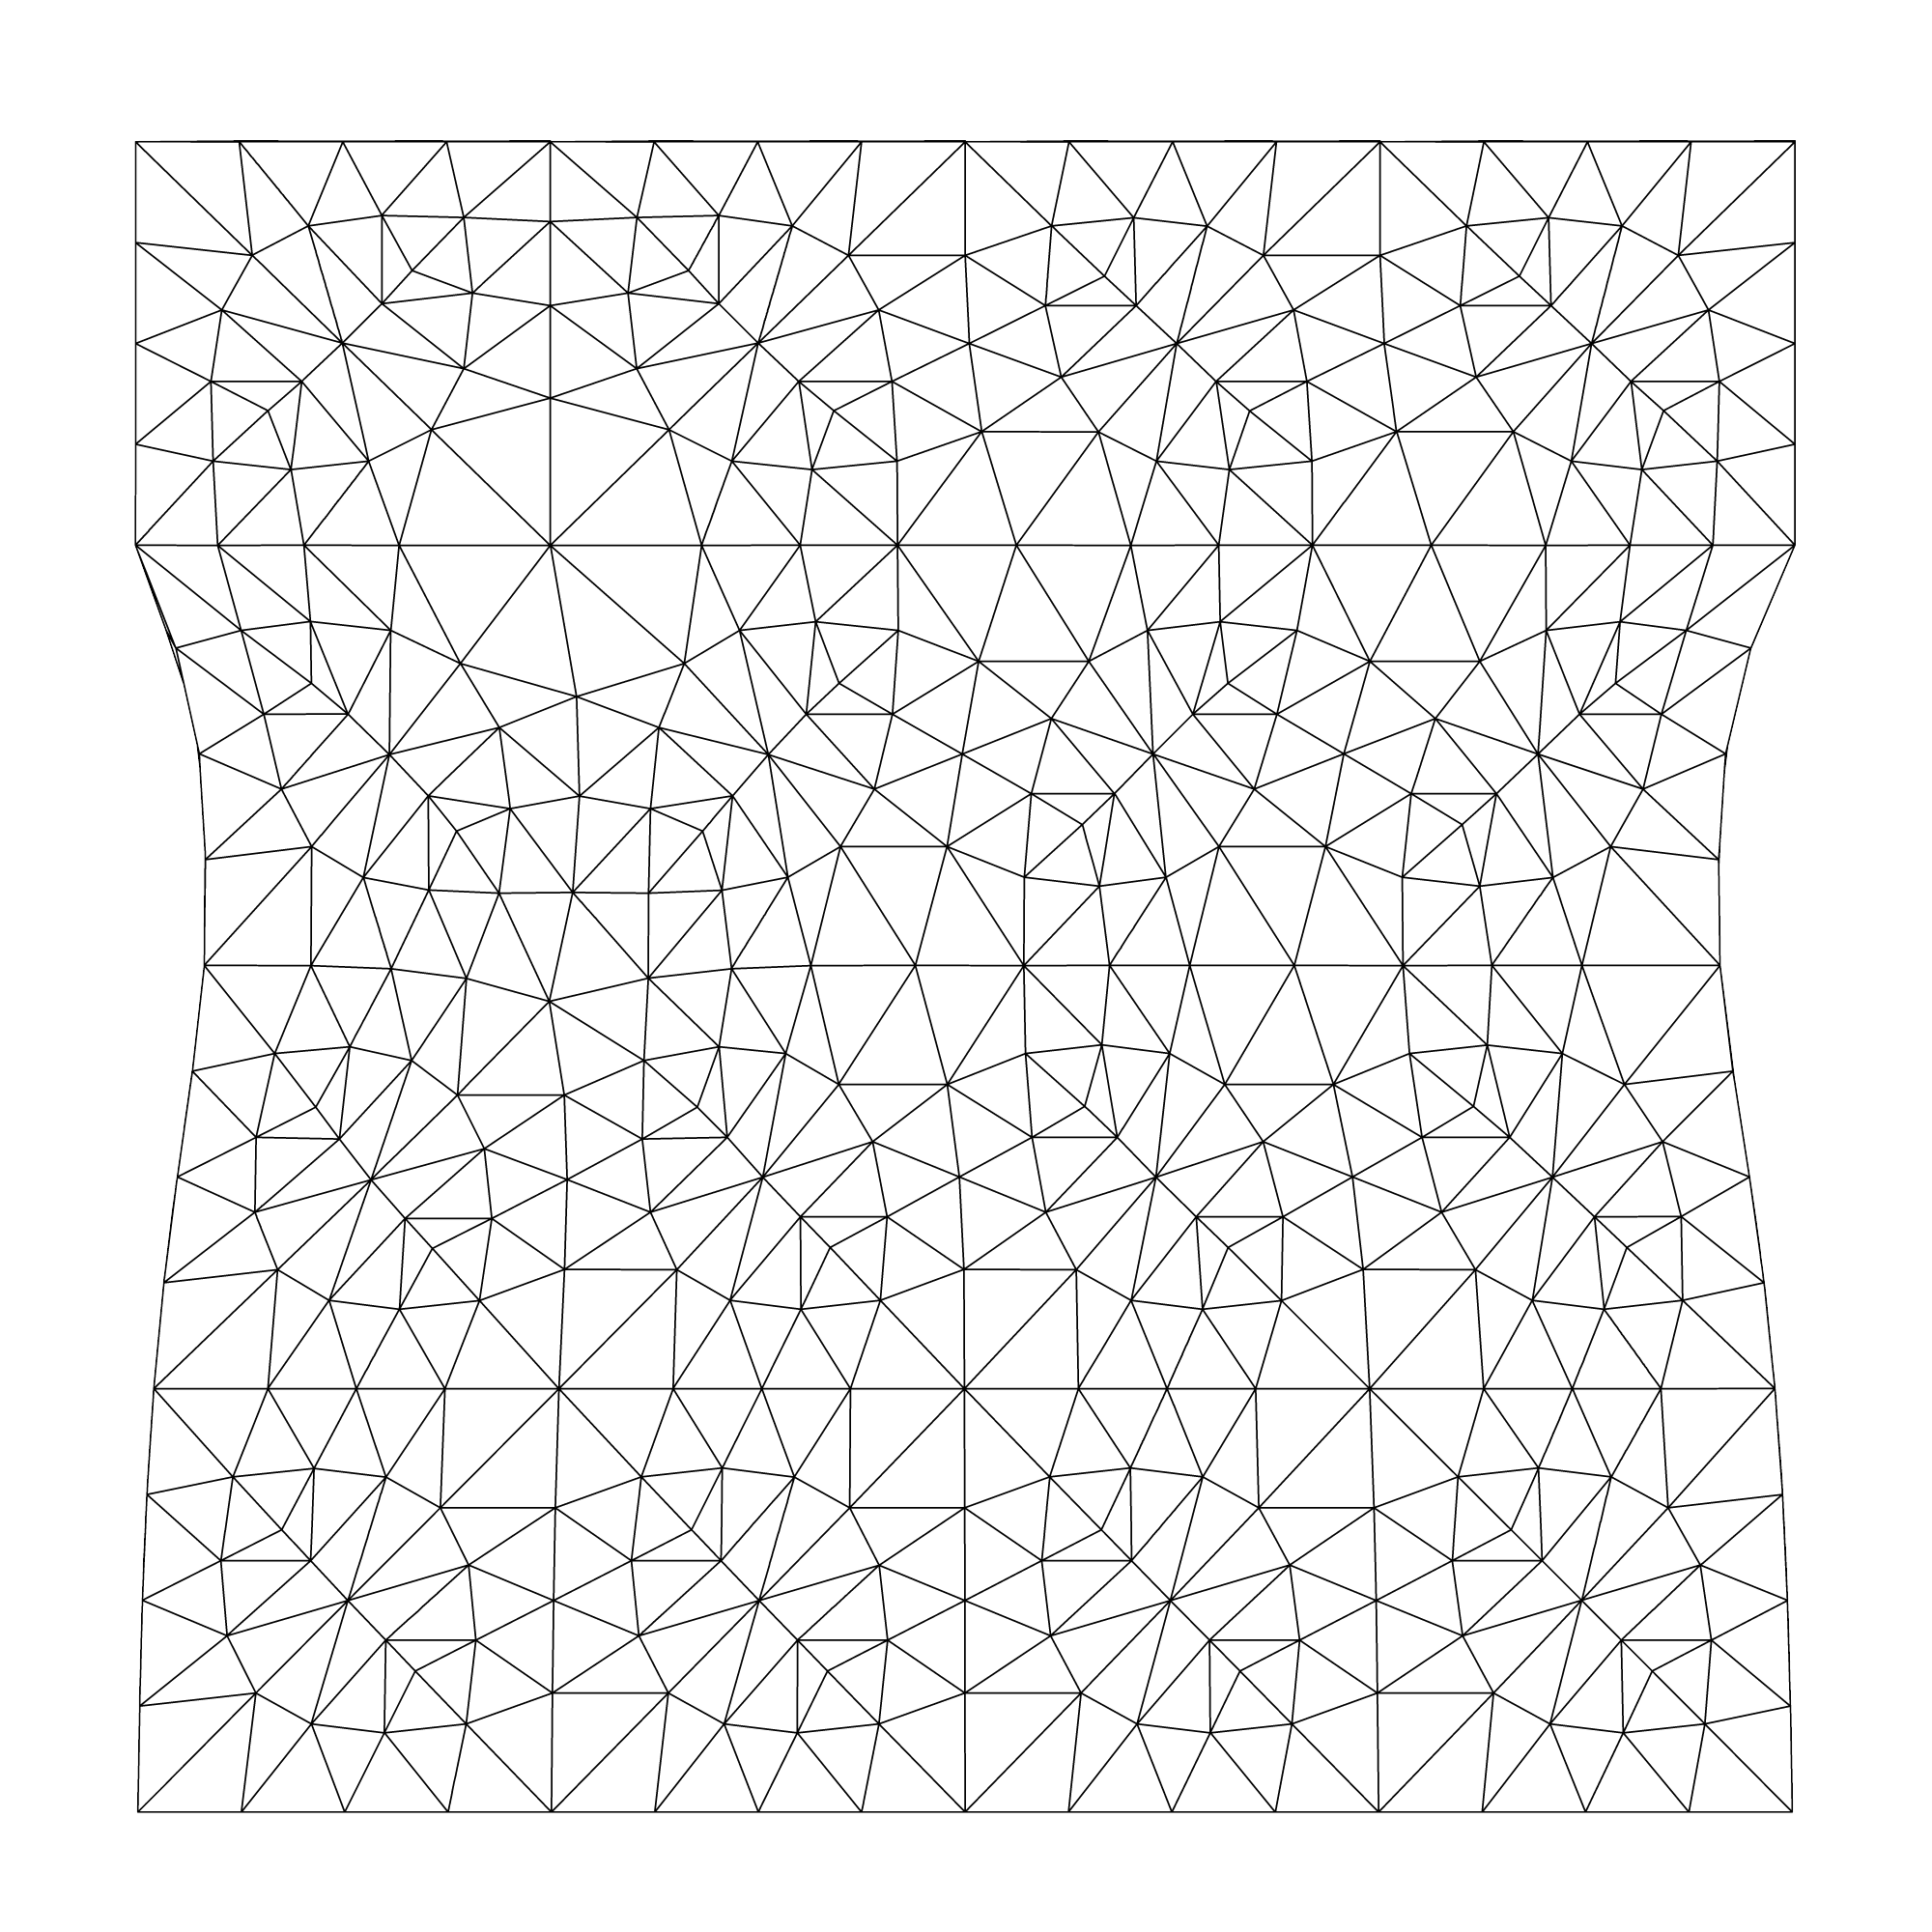
\includegraphics[width=0.4\textwidth]{../figures/lagrangian_mesh_movement_002.png} 
 \\

	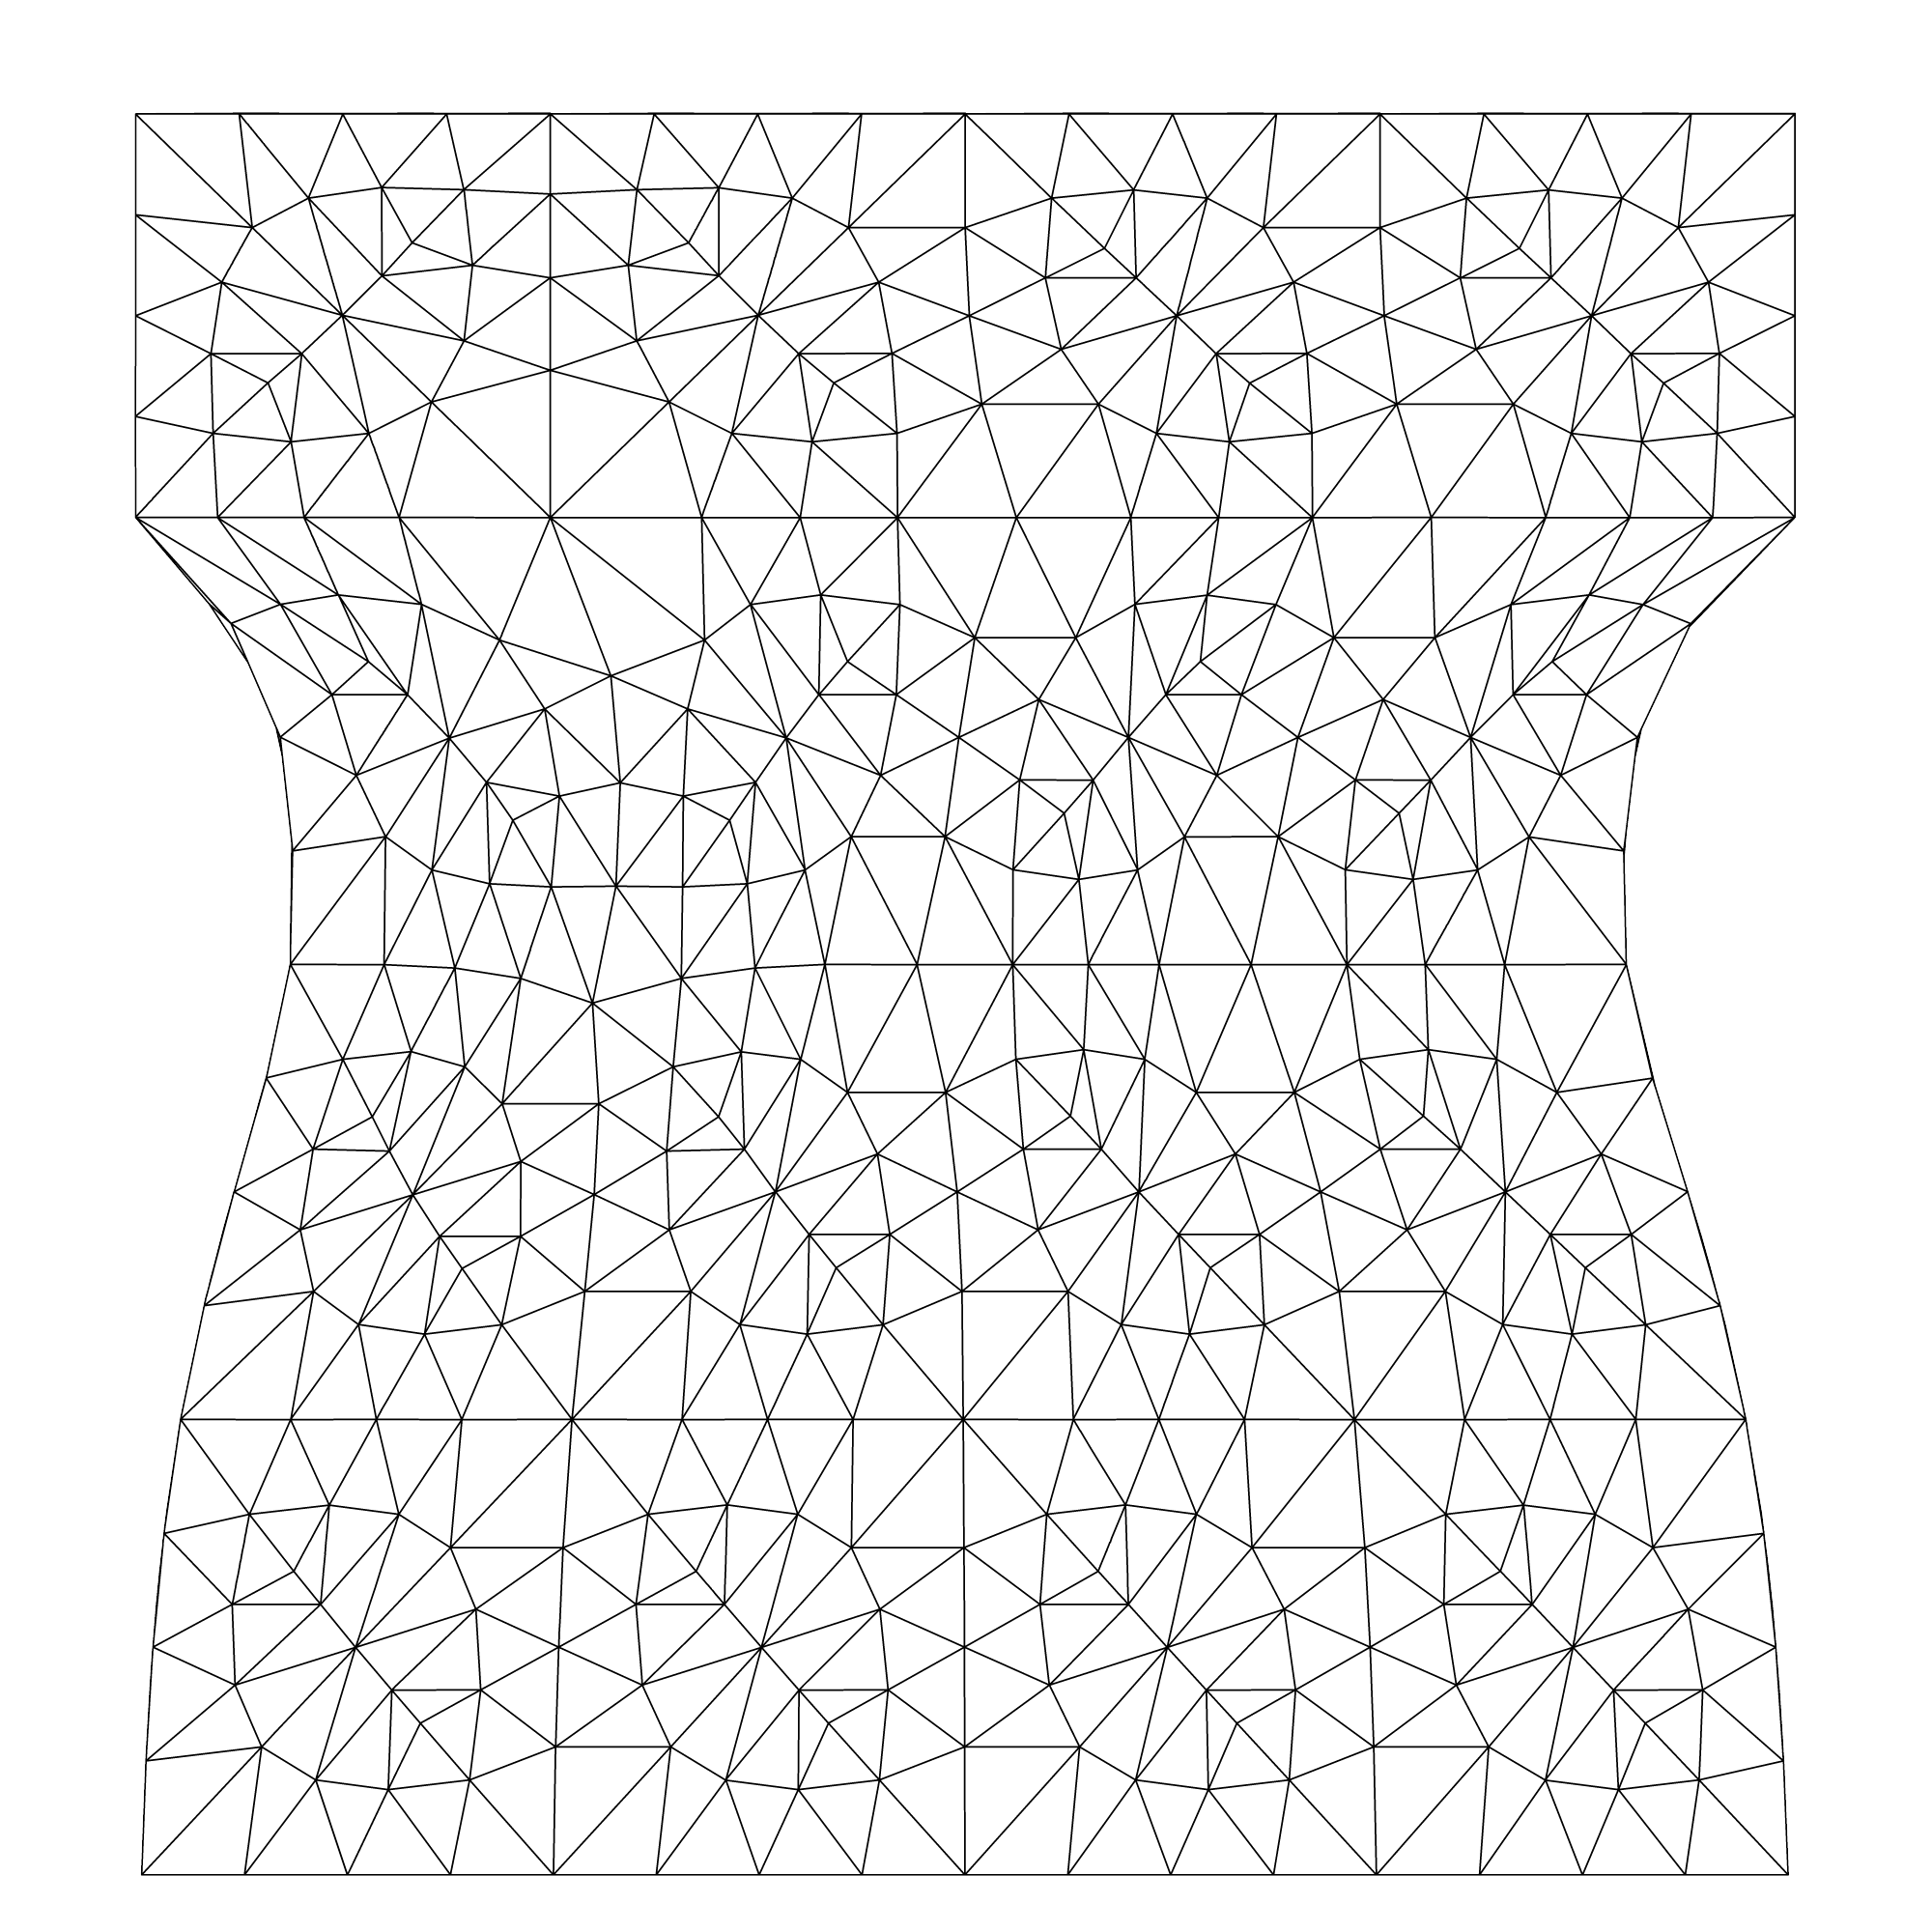
\includegraphics[width=0.4\textwidth]{../figures/lagrangian_mesh_movement_003.png} 
 &  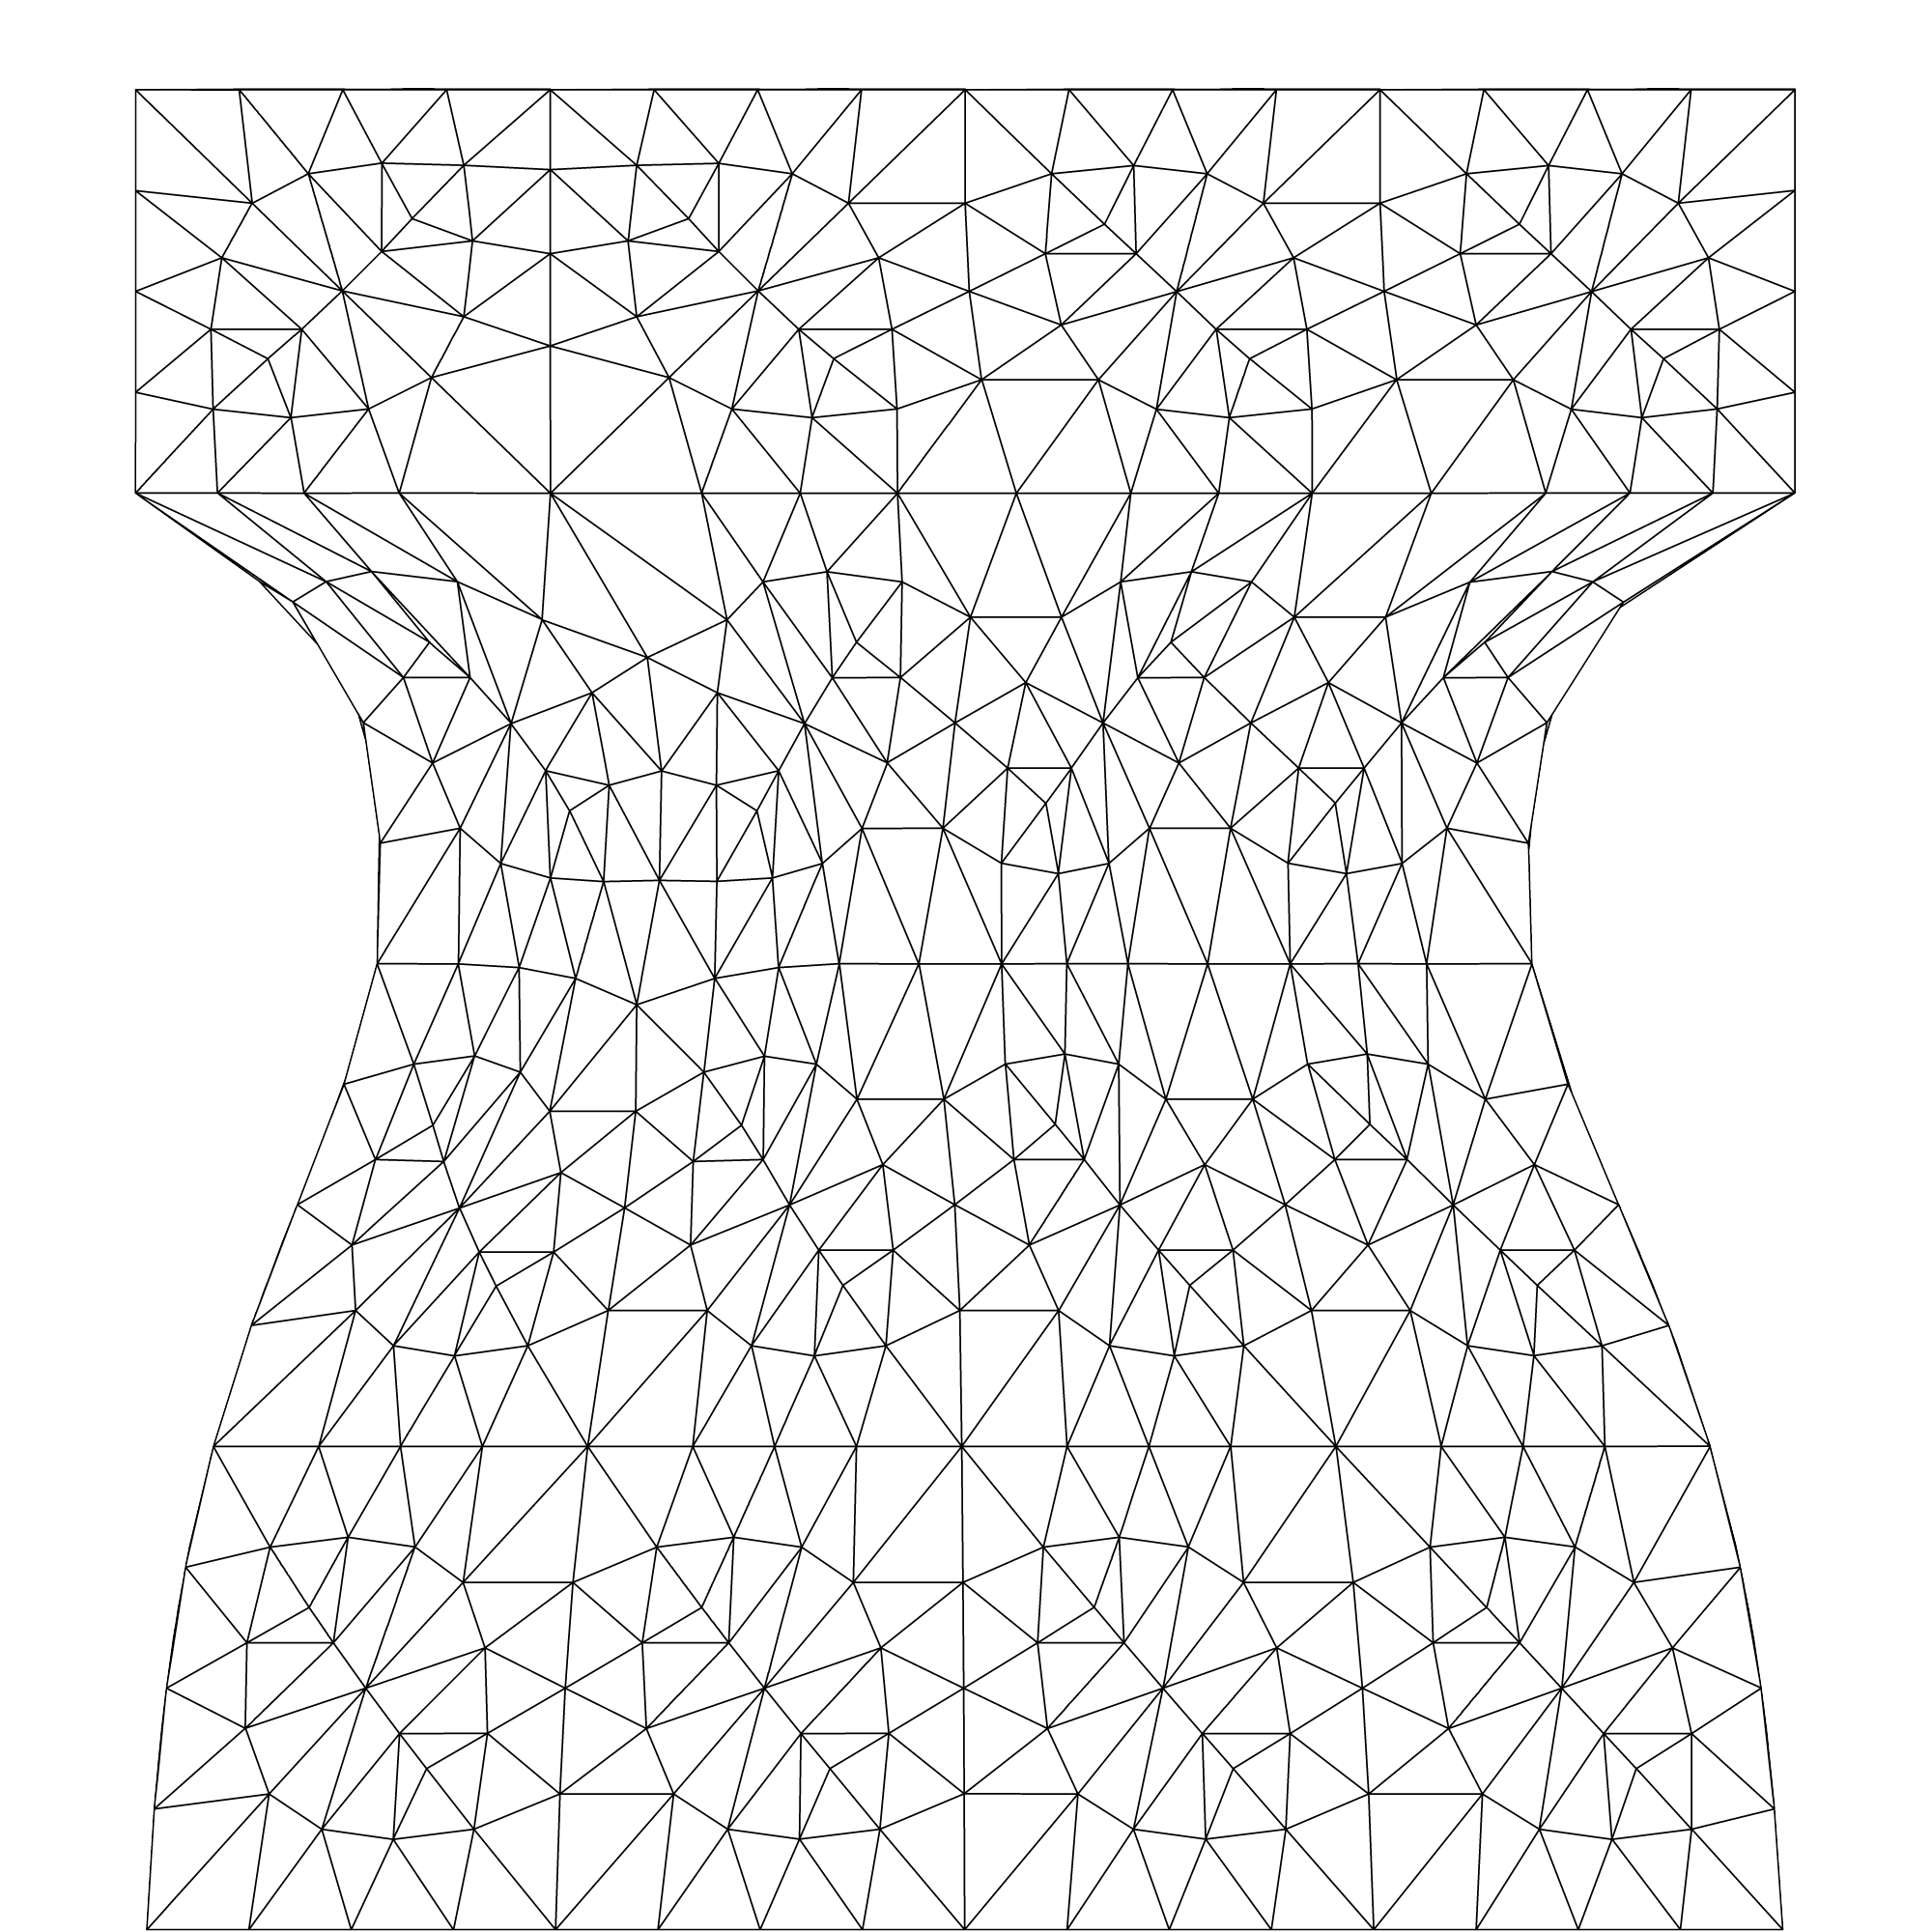
\includegraphics[width=0.4\textwidth]{../figures/lagrangian_mesh_movement_004.png}  
 \\

\end{tabular}
\caption[bla]%
{Movement of Lagrangian Mesh  during deformation \protect\footnotemark}
\label{fig:LagMesh}
\end{figure}
\footnotetext{Illustration created in Autodesk Maya.}


\section{Further Reading}
Alongside the already given literature in this Chapter, Wohlmuth2001 and Hirsch2007 give a in-depth view into discretization.

\section{Chapter passage}
With the now established general knowledge of spatial discretization and mesh types, the following Chapters
will describe the actual discretization methods and the mathematical details behind them.